\chapter[Referencial Teórico]{Referencial Teórico}

\section{Plataforma \textit{Android}}

	O \textit{Android} começou a ser desenvolvido em 2003 na empresa de mesmo nome, fundada por Andy Rubin, na qual foi adquirida em 2005 pela empresa \textit{Google}. A \textit{Google} criou a \textit{Open Handset Alliance}, que junta várias empresas da indústria das telecomunicações, como a \textit{Motorola} e a \textit{Samsung}, por exemplo. Assim, elas desenvolveram o \textit{Android} como é conhecido hoje, o qual é um sistema operacional  \textit{open source} para dispositivos móveis (baseado no \textit{kernel} do \textit{Linux}), tendo a primeira versão beta lançada em 2007 e hoje é o sistema operacional para \textit{mobile} mais utilizado.

	 De acordo com \cite{android2013}, em 2012 mais de 3,5 \textit{smartphones} com \textit{Android} eram enviados aos clientes para cada \textit{iPhone}. Em 2011, 500.000 novos \textit{devices} eram atividados a cada dia e em 2013, os números chegam a 1,5 milhões. O \textit{Android} também possui um mercado centralizado em cada aparelho (\textit{tablet} ou \textit{smartphone}) chamado \textit{Google Play}, facilitando a publicação de aplicativos. 
	O \textit{Android}  possui diferentes versões, sendo elas mostradas na Tab. (\ref{androidTab}) abaixo.  As versões mais novas possuem mais \textit{features} que as anteriores: a versão \textit{Jelly Bean}, por exemplo, possui a busca por voz que a versão \textit{Ice Cream Sandwich} não possuía. 

\begin{table}[h]
	\centering	
	\begin{tabular}{cc}
		\toprule
		\textbf{Número da versão} & \textbf{Nome}  \\
		\midrule
		1.5 &  \textit{Cupcake} \\
		1.6 & \textit{Donut} \\
		2.0/2.1 &  \textit{Éclair} \\
		2.2 & \textit{FroYo} \\
		2.3 &  \textit{Gingerbread} \\
		3.0/3.1/3.2 & \textit{HoneyComb} \\
		4.0 & \textit{Ice Cream Sandwich} \\
		4.1/4.2 & \textit{Jelly Bean} \\
		4.4 &  \textit{KitKat} \\

		\bottomrule
	\end{tabular}
	\caption{ Versões da plataforma \textit{Android}}
	\label{androidTab}
\end{table}

	Com o intuito de desenvolver para a plataforma \textit{Android}, uma das alternativas é utilizar a ferramenta \textit{Eclipse} (Fig. \ref{eclipse}) , que é um \textit{Integrated development environment} (IDE) \textit{open source}. Adicionalmente, é preciso, de acordo com \cite{androidsdkmanager}, instalar o \textit{Android Software Development Kit} e o	\textit{plugin} \textit{Android Development Tools} (ADT), que permitem desenvolver e depurar aplicações pra \textit{Android}. Outra alternativa é utilizar o \textit{Android Studio}, lançado recentemente (2013) pela empresa \textit{Google}, que já vem com todos os pacotes e configurações necessárias para o desenvolvimento, incluindo o  \textit{Software Development Kit} (SDK), as ferramentas e os emuladores. 

	\begin{figure}[h]
	\centering
		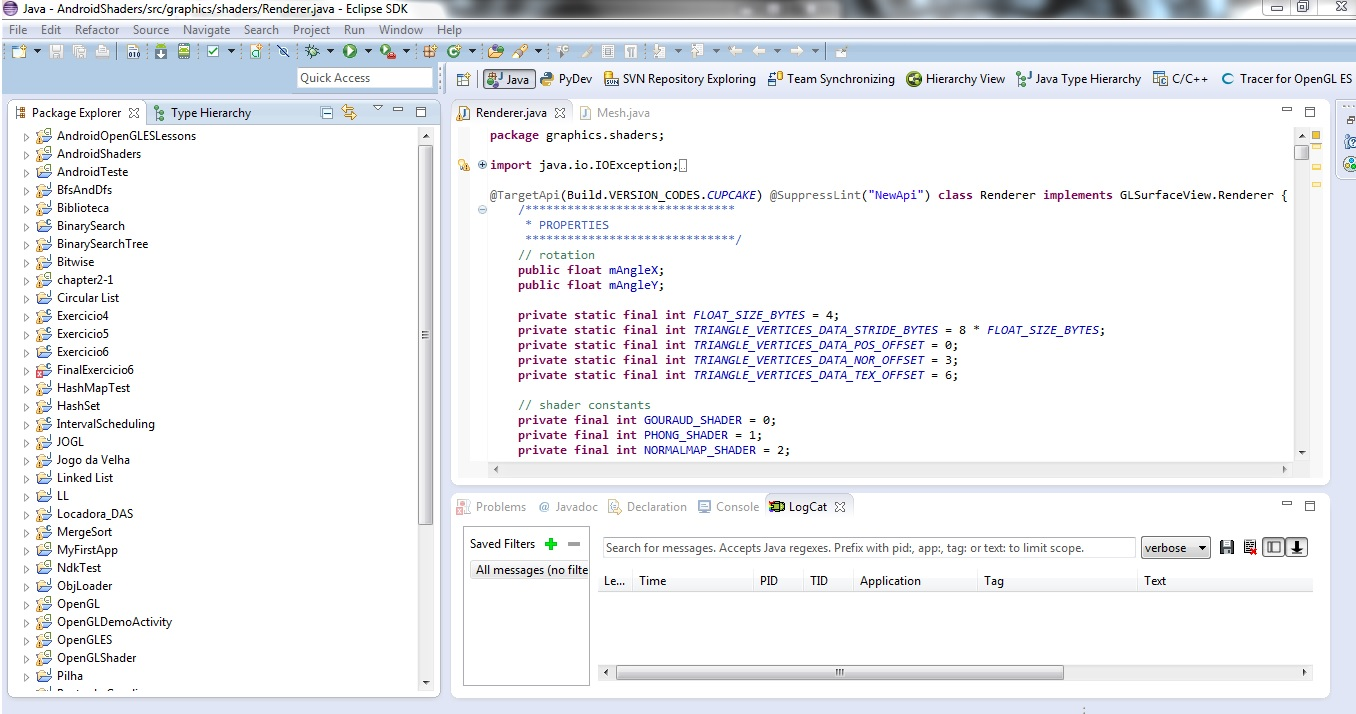
\includegraphics[keepaspectratio=true,scale=0.5]{figuras/eclipse.jpg}
	\caption{Ambiente de desenvolvimento \textit{Eclipse}}
	\label{eclipse}
	\end{figure}

\section{Bibliotecas Gráficas}

\begin{description}

	\item \textbf{2.2.1 \textit{OpenGL}}


	A \textit{OpenGL} é uma \textit{Application Programming Interface} (API) utilizada em computação gráfica para modelagem tridimensional lançada em 1992 e segundo  \cite{opengl2011}, sua precursora foi a biblioteca \textit{Integrated Raster Imaging System Graphics Library} (Iris GL) da empresa \textit{Silicon Graphics}. Ela é uma API procedural, na qual é preciso descrever os passos que involvem diversos comandos \textit{OpenGL} necessários para se chegar no efeito visual desejado. 

	Ela possui comandos para desenho de primitivas (como linhas e pontos, por exemplo), texturização, transparência, animação,  entre outros efeitos especiais.  Porém, ela não possui funções de gerenciamento de janela, eventos de \textit{input} (de \textit{mouse} e teclado, por exemplo) ou leitura e escrita de arquivos: o próprio programador é responsável por configurar o ambiente necessário para a \textit{OpenGL} desenhar em uma janela (seja para \textit{Microsoft Windows}, \textit{Mac OS} ou \textit{Unix}, por exemplo). 

	A \textit{OpenGL} possui quatro versões, sendo a mais atual a 4.4. As principais modificações ocorreram entre a 1.x para 2.x - que permitiu o uso de \textit{shaders} e \textit{pipeline} de renderização programável - e entre a 2.x e 3.x, que deprecia as funções fixas (que serão removidas nas versões posteriores). 
 
	\item \textbf{2.2.2 \textit{Glut}}

	Visando a portabilidade e abstração do sistema operacional, a biblioteca \textit{OpenGL Utility Toolkit} (Glut) foi criada por Mark Kilgard, enquanto ele ainda trabalhava na empresa \textit{Silicon Graphics}. Ela facilita a utilização de janelas e \textit{input}, integrando as janelas do sistema operacional subjacente com a  \textit{OpenGL} de forma portável entre diferentes sistemas operacionais. Embora possua limitações de \textit{Graphical User Interface} (GUI), de acordo com  \cite{opengl2011}, ela é simples de ser utilizada. 

	\item \textbf{2.2.3 \textit{OpenGL ES}}
	
	A \textit{OpenGL for Embedded Systems} (\textit{OpenGL ES}) foi lançada em 2003, e como citado em \cite{guha2011}, atualmente é uma das API's mais populares para programação de gráficos tridimensionais em pequenos \textit{devices}, sendo adotada por diversas plataformas como \textit{Android}, \textit{IOS}, Nintendo DS e \textit{Black Berry}. Segundo \cite{opengles2012}, ela possui três versões, a 1.x que utiliza as funções fixas de renderização, a 2.x, que elimina as funções fixas e foca nos processos de renderização manipulados por \textit{pipelines} programáveis e a 3.x, que é completamente compatível com a  \textit{OpenGL} 4.3.  


\end{description}

\section{Processo do \textit{Rendering Pipeline}}


	Uma cena é composta por objetos, que por sua vez são compostos por primitvas como triângulos, quadrados, linhas, por exemplo, que são constituídas de vértices, estabelecendo a geometria. Todos estes vértices seguem um processo similar de processamento para formarem uma imagem na tela.  Este processo pode ser divido em dois processos principais: o de geometria e o de rasterização.  Segundo \cite{realtime}, o processo de geometria pode ser divido nas etapas mostradas na Fig. \ref{geometria}.

	\begin{figure}[h]
	\centering
		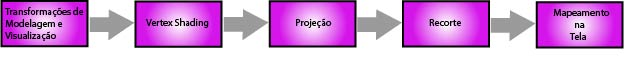
\includegraphics[keepaspectratio=true,scale=0.8]{figuras/geometria.jpg}
	\caption{Etapas do processo de geometria}
	\label{geometria}
	\end{figure}

	Na etapa Transformações de Modelagem e Visualização, as coordenadas do objeto são transformadas, de forma que ele possa ser posicionado, orientado e tenha um tamanho determinado. Após essa etapa, é dito que o objeto está localizado no espaço do mundo e é aplicada a transformação de visualização, que tem como objetivo estabelecer a câmera na origem, mirando em direção ao eixo z negativo. 

	A próxima etapa é a de \textit{Vertex Shading}, responsável por modelar parte dos efeitos (a outra parte é feita durante a rasterização), pois renderizar somente a forma e posição não é suficiente.  Estes efeitos incluem os materiais dos objetos, como também os efeitos da luz, podendo ser modelados de diferentes formas, como representações de descrições físicas. Muitos dados sao armazenados em cada vértice, como a sua localização e normal, por exemplo. Assim, os resultados do \textit{vertex shading} são mandados para o estágio de rasterização para serem interpolados. 

	A Projeção é responsável por transformar o volume de visualização aplicando métodos de projeção, como a perspectiva e a ortográfica (também chamada de paralela). A projeção ortográfica resulta em uma caixa retangular, em que linhas paralelas permanecem paralelas após a transformação. Na perspectiva, quanto mais longe um objeto se encontra, menor ele aparecerá após a projeção e linhas paralelas tendem a convergir no horizonte. Ela resulta em um tronco de pirâmide com base retangular. 

	Somente as primitivas gráficas que se encontram dentro do volume de visualização que serã renderizadas. Assim, o recorte (chamado de \textit{clipping}) é responsável por não passar adiante as primitivas que se encontram fora da visualização. Primitivas que estão parcialmente dentro, são recortadas, ou seja, o vértice que está de fora não é renderizado e é substituído por um novo vértice (dentro do volume de visualização). A  Fig. \ref{clip} mostra esta ideia.

       \begin{figure}[h]
       \centering
	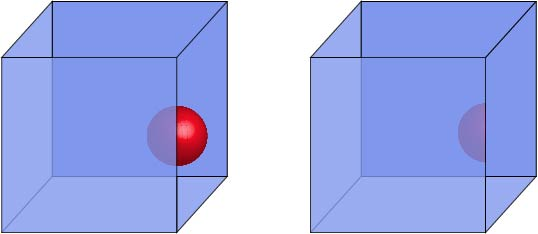
\includegraphics[keepaspectratio=true,scale=0.8]{figuras/clip.jpg}
       \caption{Antes do recorte (cubo de visualização esquerdo) e depois do recorte (cubo de visualização direito)}
       \label{clip}
       \end{figure}


	A última etapa de geometria é a de mapeamento na tela, em que a entrada são as primitivas recortadas e as coordenadas ainda são tridimensionais. Assim, esta etapa tem como finalidade mapear as coordenadas tridimensionais em coordenadas de tela. Para isto, o centro de um \textit{picture element} (\textit{pixel}) é igual a coordenada 0,5. Então, \textit{pixels} de [0; 9] equivalem à cobertura das coordenadas de [0,0; 10,0). E os valores dos \textit{pixels} crescem da esquerda para a direita e de cima para baixo.

	Terminado o processo de geometria, o próximo a ser feito é o de rasterização, em que seu objetivo é computar e definir as cores para cada \textit{pixel}. Este processo pode ser dividido em quatro etapas mostradas na Fig. \ref{rasteriza}.

   \begin{figure}[h]
       \centering
	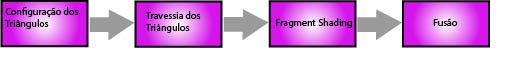
\includegraphics[keepaspectratio=true,scale=0.8]{figuras/rasteriza.jpg}
       \caption{Etapas do processo de rasterização}
       \label{rasteriza}
       \end{figure}

	Na etapa de Configuração dos Triângulos, as diferenciais e outros dados são computados para as superfícies dos triângulos. Estes dados serão utilizados para a conversão dos dados vindos do processo de geometria (coordenadas e suas informações provenientes do \textit{vertex shader}) em \textit{pixels} na tela e também para o processo de interpolação. 

	A Travessia de Triângulos checa se cada um dos \textit{pixels} está dentro de um triângulo ou não. Para cada \textit{pixel} que sobrepõe um triângulo, um fragmento é gerado como mostrado na Fig. \ref{traversal}. Cada fragmento tem a informação sobre sua localização na tela, no triângulo e sua profundidade e as propriedades dos fragmentos dos triângulos são geradas usando dados interpolados entre os três vértices do triângulo. 

  \begin{figure}[h]
       \centering
	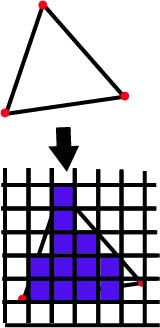
\includegraphics[keepaspectratio=true,scale=0.8]{figuras/traversal.jpg}
       \caption{Travessia de triângulos: fragmentos sendo gerados}
       \label{traversal}
       \end{figure}

	As computações por \textit{pixel} são calculadas durante o \textit{fragment shading}, em que o resultado é uma ou mais cores a serem passadas para o próximo estagio. Muitas técnicas podem ser aplicadas durante esta etapa e uma das mais importantes é a de texturização (que aplica no fragmento do objeto parte de uma imagem). 

	 A informação relacionada com cada \textit{pixel} é armazenada no \textit{color buffer}, que é um \textit{array} de cores. Assim, a última etapa é a de fusão, que é responsável por combinar a cor do fragmento gerada pelo estágio anterior com a cor armazenada no \textit{buffer}. Ela também é responsável pela visibilidade, em que o \textit{color buffer} deve conter as cores das primitivas da cena que são visíveis do ponto de vista da câmera. Isto é feito através do Z-\textit{buffer} (também chamado de \textit{buffer} de profundidade), que para cada \textit{pixel} armazena a coordenada z a partir da câmera até a primitiva mais próxima.  Então, a coordenada z de uma primitiva que está sendo computada é comparada com  o valor do Z-\textit{buffer} para o mesmo \textit{pixel}. Se o valor for menor, quer dizer que a primitiva esta mais próxima da câmera do que o valor da anterior, e assim, o valor do Z-\textit{buffer} é atualizado para o atual. Se o valor corrente for maior, então o valor do Z-\textit{buffer} não é modificado. 

\section{Renderizando Modelos Tridimensionais}

\begin{description}	
	\item \textbf{2.4.1 Função Fixa}

	As versões da \textit{OpenGL} anteriores a 3.0  e a versão 1.0 da \textit{OpenGL ES} permitem a utilização de funções fixas para a renderização, ou seja, as funções da API em \textit{pipeline} estático. As vantagens das funções fixas é que elas são mais convenientes, assim, um programador com pouca experiência em  \textit{OpenGL} ou \textit{OpenGL ES} podem ter uma aprendizagem mais rápida. Em contrapartida, este método não dá flexibilidade ao programador de moficiar algumas das etapas de renderização (vistas na Seção 2.3). 

	 Uma das operações fixas é para a de desenho de objetos, em que se utiliza a chamada \textit{glVertex3f(float x, float y, float z)} (entre as declarações \textit{glBegin(Glenum mode} e \textit{glEnd()}) para se desenhar um objeto. \textit{Mode} diz qual primitiva deve ser utilizada, podendo ser: pontos; linhas; série de linhas conectadas; série de linhas conectadas (em que conectam-se também o primeiro e último vértices); triângulos; série de triângulos conectados; quadriláteros; série de quadriláteros e polígonos convexos simples. 

	Para se definir a cor, utiliza-se o  comando \textit{glColor3f(float r, float g, float b)}, em que os argumentos são as coordenadas do modelo Red Green and Blue (RGB) e neste modelo, define-se cada cor pela quantidade de vermelho, verde e azul que a compõei. Um argumento a mais pode ser adicionado (utilizando-se o comando \textit{glColor4f(float r, float g, float b, float alpha)}), em que o argumento \textit{alpha} é o valor de transparência (1,0 é considerado a sua intensidade total).  

	Outras funções existentes são as de definição da projeção, utilizando \textit{glOrtho(GLdouble left, GLdouble right, GLdouble bottom, GLdouble top, GLdouble near, GLdouble far} para projeções ortográficas ou \textit{glFrustum(GLdouble left, GLdouble right, GLdouble bottom, GLdouble top, GLdouble near, GLdouble far} para perspectiva. O significados dos parâmetros, segundo \cite{guha2011}, podem ser vistos nas  Fig. \ref{ortopers}.


 	\begin{figure}[h]
	\centering
		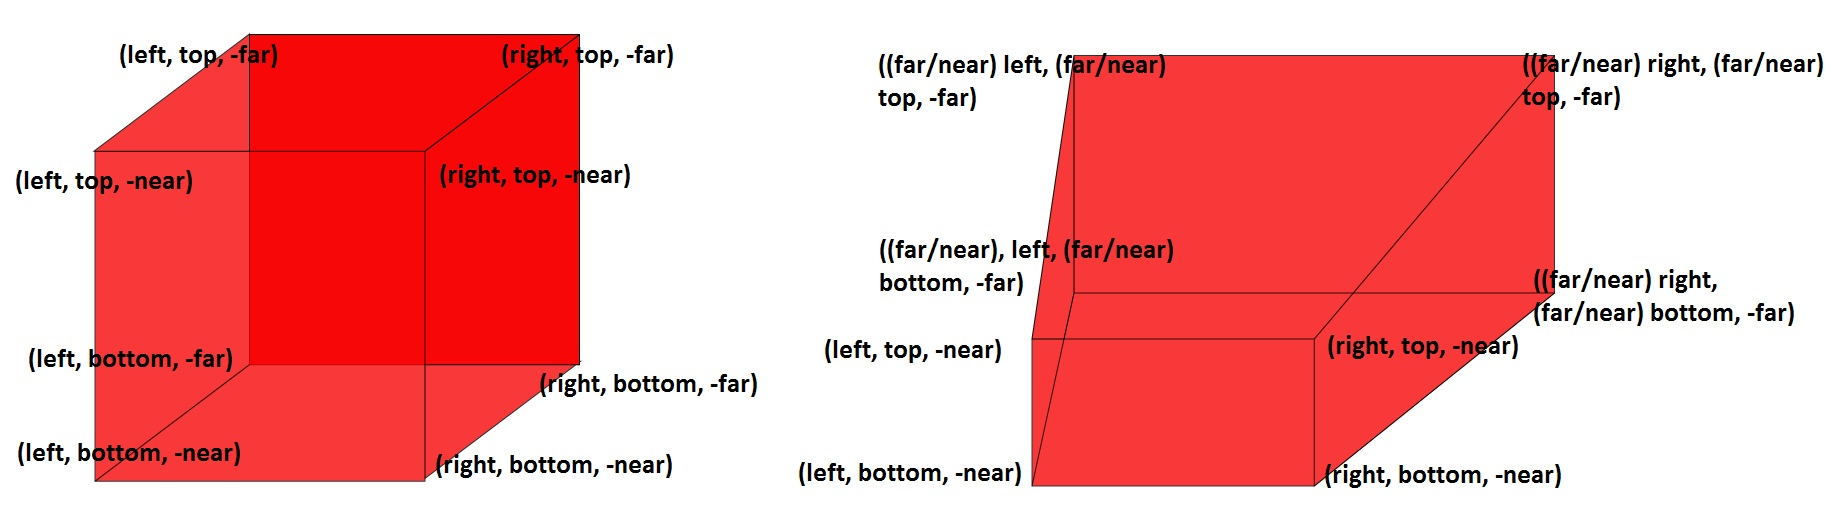
\includegraphics[keepaspectratio=true,scale=0.35]{figuras/ortopers.jpg}
	\caption{Projeção Ortográfica: parâmetros}
	\label{ortopers}
	\end{figure}

	\item \textbf{2.4.2 \textit{Vertex Array}}

	Um modelo tridimensional pode ser descrito por uma lista de vértices e uma lista de índices. Na Fig. \ref{quadrado}, tem-se dois triângulos e quatro vértices definidos (dois vértices são compartilhados). Assim, pode-se definir um vetor com os vértices [v0, v1, v2, v3] e um vetor de índices [0, 3, 1, 0, 2, 3], que diz a ordem que os vértices devem ser renderizados. 

	\begin{figure}[h]
	\centering
		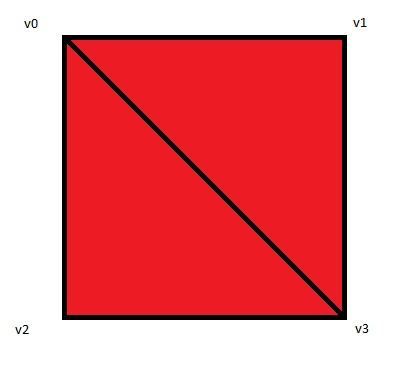
\includegraphics[keepaspectratio=true,scale=0.5]{figuras/quadrado.jpg}
	\caption{Vértices do quadrado constituído de dois triângulos}
	\label{quadrado}
	\end{figure}


	Segundo  \cite{guha2011}, as coordenadas dos vértices podem ser armazenadas em um vetor e passadas para a \textit{OpenGL} como um ponteiro. O vetor de vértices é ativado com a chamada \textit{glEnableClientState(G\_VERTEX\_ARRAY)} e o ponteiro é definido através da função \textit{glVertexPointer(size, type, stride, *pointer)}. O parâmetrro \textit{pointer} é o endereço de onde começa o vetor, \textit{type} é o tipo dos dados, \textit{size} é o número de valores por vértice e \textit{stride} é o \textit{offset} em \textit{bytes} entre o início dos valores para sucessivos vértices (zero indica que os valores para os vértices sucessivos não estão separados). Com o \textit{stride} é possível armazenar os vértices de posição e normais em único vetor, por exemplo. 

	Finalmente, a renderização pode ser feita por meio da chamada \textit{glDrawElements(primitive, count, type, *indices)}, em que \textit{primitive} é a primitiva geométrica (pontos, linhas, triângulos, por exemplo), \textit{type} é o tipo de dado, \textit{indices} é o vetor de índices e \textit{count} é o número de índices a serem usados. 

	Dessa forma, os dados são definidos em apenas um local, podendo ser utilizados em vários locais do código, evitando redundância e também diversos dados (como coordenadas de posição, textura, normais, por exemplo) podem ser definidos em um único vetor, sendo mais eficiente.     

	\item \textbf{2.4.3 \textit{Vertex Object Buffer}}	

	A ideia do \textit{Vertex Object Buffer} é a mesma do \textit{Vertex Array}, porém de acordo com \cite{vbo}, o \textit{driver} gráfico pode optar por colocá-lo diretamente na memória da GPU, melhorando o desempenho para objetos que não são modificados com muita frequência. 

	Primeiramente é necessário criar um novo \textit{buffer} e para isso, de acordo com \cite{interactive2012}, é necessário utilizar a chamada\textit{glGenBuffers()}. Feito isto, vincula-se o vetor ao \textit{buffer} com a fução \textit{glBindBuffer(GLenum  target, GLint id)}, em que \textit{target} é o tipo do \textit{buffer} (GL\_ARRAY\_BUFFER, por exemplo) e \textit{id} é o identificador. Para fazer uma cópia dos dados do vetor ao \textit{buffer}, utiliza-se a \textit{glBufferData(GLenum target, GLsizeptr size, const GLvoid *data, GLenum usage)}, em que \textit{target} é o tipo, \textit{size} é o tamanho em \textit{bytes} do \textit{buffer}, \textit{data} é o ponteiro para os dados que serão copiados e \textit{usage} é o padrão de utilização dos dados. Os padrões e seus significados podem ser vistos na Tab. (\ref{bufferdata}.

\begin{table}[h]
	\centering	
	\begin{tabular}{cc}
		\toprule
		\textbf{Padrão} & \textbf{Significado}  \\
		\midrule
		\textit{GL\_STREAM\_DRAW} &  O objeto será modificado apenas uma vez e usado poucas vezes  \\
		\textit{GL\_STATIC\_DRAW} & O objeto será modificado uma vez, mas será usado várias vezes \\
		\textit{GL\_DYNAMIC\_DRAW} &  O objeto será modificado e usado várias vezes \\
		\bottomrule
	\end{tabular}
	\caption{ Palavras-chave do formato obj}
	\label{bufferdata}
\end{table}

	Após a cópia dos dados, deve-se garantir que eles serão desvinculados do \textit{buffer} utilizando novamente a \textit{glBindBuffer()}, mas dessa vez o parâmetro \textit{id} como zero. Além disso, é necessário utilizar a chamada \textit{glDeleteBuffers(GLsizei n, const GLuint * buffers)} (em que n é o número de objetos do \textit{buffer} e \textit{buffer} é o array de \textit{buffers} a serem deletados) para poder liberar a memória. Os mesmos procedimentos podem ser feitos para criar o \textit{buffer} de índices. 
  

	\item \textbf{2.4.4 Formato obj}

	Em uma cena, os modelos tridimensionais podem variar muito mais do que formas básicas como uma esfera e um torus, por exemplo. Assim, o formato obj foi criado pela empresa  \textit{Wavefront} e é um arquivo para leitura de objetos tridimensionais, a fim de carregar geometrias mais complexas. Segundo \cite{graphicsprog}, neste arquivo cada linha contém informações a respeito do modelo, começando com uma palavra-chave, seguida da informação. A  Tab. (\ref{palavraschave}) mostra as principais palavras-chave utilizadas. 

\begin{table}[h]
	\centering	
	\begin{tabular}{cc}
		\toprule
		\textbf{Palavra-chave} & \textbf{Significado}  \\
		\midrule
		\textit{usemtl} & Indica se está utilizando material  \\
		\textit{mtlib} &  Nome do material \\
		v &  Coordenadas x, y e z do vértice \\
		vn & Coordenadas da normal \\
		vt &  Coordenadas da textura \\
		f &  Face do polígono \\
		\bottomrule
	\end{tabular}
	\caption{ Palavras-chave do formato obj}
	\label{palavraschave}
\end{table}

	A face do polígono (f) possui três índices que indicam os vértices do triângulo. Assim, cada vértice possui um índice (que depende de quando ele foi declarado), começando a partir de um. A Fig. \ref{objFile} mostra o exemplo de um arquivo obj para a leitura de um cubo. 

	\begin{figure}[h]
	\centering
		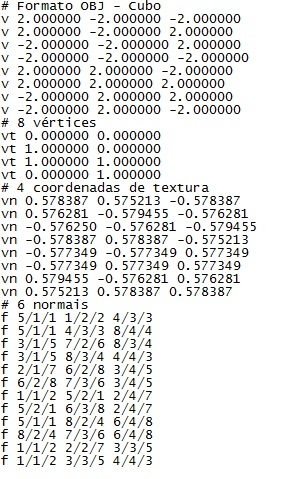
\includegraphics[keepaspectratio=true,scale=0.9]{figuras/obj.jpg}
	\caption{Arquivo obj de um cubo}
	\label{objFile}
	\end{figure}

	Então, a partir da leitura do arquivo obj, é possível ler cada linha e armazenar em estruturas de dados, as informações que serão passadas para renderizar o modelo tridimensional, como vértices e índices. 

\end{description}

\section{Quadros Por Segundo}

	\textit{Frame rate} é o quão rápido uma sequência de \textit{frames}, ou quadros, são apresentados ao espectador. A unidade utilizada para determinar \textit{frame rate} em jogos e filmes são os \textit{frames per second} (FPS) ou quadros por segundo, que é o número de imagens renderizadas por segundo. O tempo usado por uma aplicação para gerar uma imagem varia dependendo da complexidade da computação desempenhada durante cada quadro.  O FPS é utilizado tanto para expressar a taxa de um quadro em particular quanto para determinar o desempenho médio durante o uso da aplicação. 

	De acordo com \cite{framerate2009}, jogos na América do Norte e Japão são renderizados a 30 ou 60 quadros por segundo, porque essa é a taxa de atualização do sistema \textit{National Television System Committee} (NTSC) usadas nessas regiões. Na Europa e no resto do mundo esta taxa é de 50 quadros por segundo, pois é a taxa de atualização dos televisores do tipo \textit{Phase Alternating Line} (PAL) ou \textit{Séquentiel Couleur à Mémoire} (SECAM). Todos estes sistemas são sistemas de televisores analógicos.

\section{\textit{Shaders}: \textit{pipelines} programáveis}
	
	Conforme \cite{realtime}, \textit{shading} é o processo de utilizar uma equação para computar o comportamento da uma superfície de um objeto. Então, \textit{shaders} são programas escritos pelo programador, a fim de substituir as funcionalidades fixas e existem dois tipos de \textit{shader}, que focam diferentes partes do \textit{pipeline} gráfico: o \textit{vertex shader} e o \textit{fragment shader}. 

	O   \textit{vertex shader} é responsável pela manipulação dos dados dos vértices, incluindo coordenadas, normais, cores, sendo responsável pela alteração de posição e textura, por exemplo. Ele altera a etapa de \textit{vertex shading}, descrita na Seção 2.3. Ele deve, ao menos, definir as coordenadas de posição. 

	O \textit{fragment shader} opera nos fragmentos no processo de rasterização (selecionar e colorir os \textit{pixels}) antes de passar para a etapa de Fusão descrita na Seção 2.3, que faz as operações por fragmento (como o teste de profundidade). Ele deve, ao menos, atribuir uma cor para cada fragmento. 

	A linguagem  \textit{OpenGL Shading Language} (GLSL) foi incluída na versão 2.0 da  \textit{OpenGL}, sendo desenvolvida com o intuito de dar aos programadores o controle de partes do processo de renderização (através dos \textit{shders}), substituindo as funções fixas. A GLSL é baseada na linguagem C, mas antes de sua padronização, o programador tinha que escrever o código na linguagem \textit{Assembly}, a fim de acessar os recursos da GPU. Além dos tipos clássicos do C, \textit{float}, \textit{int} e \textit{bool}, a GLSL possui outros tipos mostrados na Tab. (\ref{tiposglsl}).

\begin{table}[h]
	\centering	
	\begin{tabular}{cc}
		\toprule
		\textbf{Tipo} & \textbf{Descrição}  \\
		\midrule
		vec2, vec3, vec4 & Vetores do tipo \textit{float} de 2, 3 e 4 entradas \\
		ivec2, ivec3, ivec4 & Vetores do tipo inteiro de 2, 3 e 4 entradas \\
		mat2, mat3, mat4 & Matrizes 2x2, 3x3 e 4x4 \\
		sampler1D, sampler2D, sampler3D & Acesso a texturas \\
		\bottomrule
	\end{tabular}
	\caption{ GLSL: tipos de dados}
	\label{tiposglsl}
\end{table}

	Além disso, a GLSL possui variáveis chamadas qualificadoras, que fazem o interfaceamento do programa e os \textit{shaders} e entre \textit{shaders}. Estas varáveis são mostradas na Tab. (\ref{tiposqualificadores}).

	\begin{table}[h]
	\centering	
	\begin{tabular}{cc}
		\toprule
		\textbf{Tipo} & \textbf{Descrição}  \\
		\midrule
		attribute &  Variável utilizada pelo programa para comunicar dados relacionados aos \\
		               &  vértices para o \textit{vertex shader}\\
		uniform &  Variável utilizada pelo programa para comunicar dados relacionados \\
			&  com as primitivas para ambos os \textit{shaders} \\
		varying &  Variável utilizada pelo \textit{vertex shader} para se comunicar \\
			& com o \textit{fragment shader} \\
		\bottomrule
	\end{tabular}
	\caption{ GLSL: qualificadores}
	\label{tiposqualificadores}
	\end{table}

\section{\textit{Flat Shading}, \textit{Gouraud Shading} e \textit{Phong Shading}}

	No método \textit{Flat Shading}, renderiza-se cada polígono de um objetdo com base no ângulo entre a normal da superfície e a direção da luz. Mesmo se as cores se diferenciem nos vértices de um mesmo polígono, somente uma cor é escolhida entre elas e é aplicada em toda o polígono.  

	A computação dos cálculos de luz nos  vértices seguida por uma interpolação linear do resultado é conhecida como \textit{Gouraud Shading} (considerada superior ao \textit{Flat Shading}), criada por Henri Gouraud, sendo conhecida como avaliação por vértice. Nela, o \textit{vertex shader} deve calcular a intensidade em cada vértice e os resultados serão interpolados, em seguida, o \textit{fragment shader} pega este valor e passa adiante. Segundo  \cite{guha2011}, é o padrão implementado pela  \textit{OpenGL}. 

	No \textit{Phong Shading}, primeiramente interpola-se os valores das normais das primitivas e então computam-se os cálculos de luz para cada \textit{pixel}, utilizando as normais interpoladas. Este método também é conhecido como avaliação por \textit{pixel}. A intensidade de luz é calculada de acordo com a equação de luz de \textit{Phong} mostrada em \cite{guha2011}.

	 A \textit{OpenGL} oferece este tipo de \textit{shading} como opção ou pode ser implementado utilizando \textit{shaders}.  Ele requer maior poder de processamento do que a técnica \textit{Gouraud Shading}, pois cálculos nos vértices são menos intensos comparados aos cálculos feitos por \textit{pixels}. Porém, a desvantagém da técnica de \textit{Gouraud Shading} é que efeitos de luz que não afetam um vértice de uma superfície não surtirão efeito, como por exemplo, efeitos de luz localizados no meio de um polígono (como um brilho, por exemplo) não serão renderizados corretamente. Porém, se o efeito ocorrer em um vértice, o \textit{Phong Shading} renderiza corretamente o vértice, mas irá interpolar erroneamente. A Fig. \ref{fgp} mostra a diferença entre as três técnicas de \textit{shading} aplicadas em uma esfera com uma luz direcional. 

	\begin{figure}[h]
	\centering
		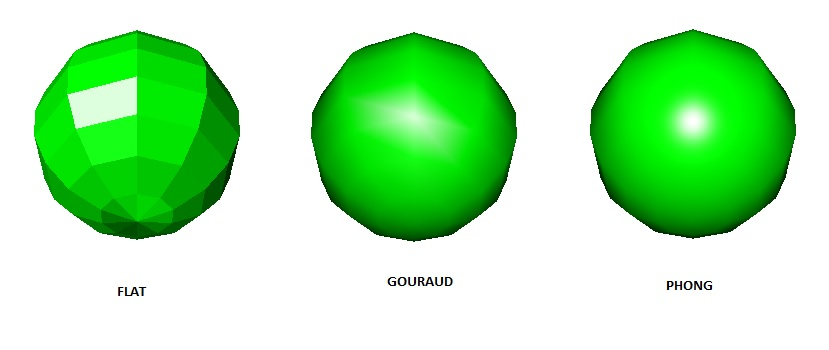
\includegraphics[keepaspectratio=true,scale=0.7]{figuras/flatgp.jpg}
	\caption{Comparação entre as técnicas de \textit{shading}}
	\label{fgp}
	\end{figure}


\section{Ferramentas}

\begin{description} 

	\item \textbf{2.8.1. \textit{Adreno Profiler}}

	A \textit{Adreno} é uma ferramenta que foca na otimização gráfica para celulares que possuem \textit{Graphics processing unit} (GPU) Adreno (fabricada pela empresa \textit{Qualcomm}). De acordo com  \cite{adp}, a ferramenta provê suporte para \textit{Android} e \textit{Windows RT} (variação do sistema operacional \textit{Windows} 8  e projetada para \textit{devices} móveis), permitindo a otimização, análise por quadros e visualização de desempenho em tempo real. 

	Como pode ser visto na Fig. \ref{adrenoProfiler}, a ferramenta possui um módulo de análise dos \textit{vertex} e \textit{fragment} \textit{shaders}, sendo possível editá-los e analisar os resultados de compilação em tempo real, além dela também gerar estatísticas.  

	\begin{figure}[h]
	\centering
		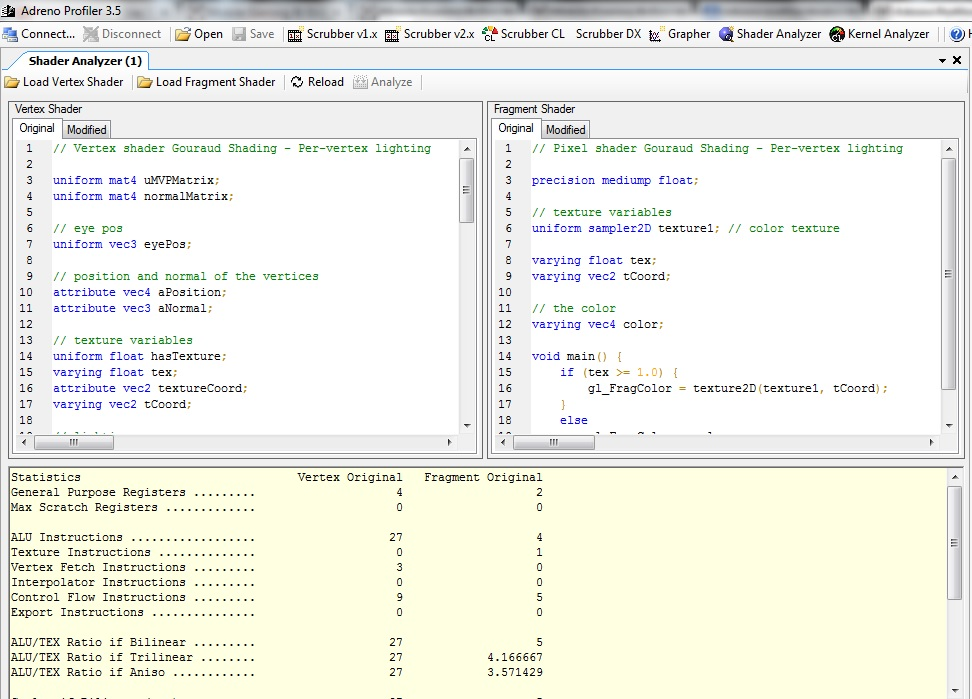
\includegraphics[keepaspectratio=true,scale=0.4]{figuras/shader_analyzer.jpg}
	\caption{Ferramenta \textit{Adreno Profiler}: analisador de \textit{shaders}}
	\label{adrenoProfiler}
	\end{figure}

	O módulo gráfico permite analisar algumas métricas, como a de quadros por segundo, em que na Fig. \ref{graph} um gráfico é plotado em tempo de execução. Além disso, ela também exporta os resultados no formato \textit{Comma-Separated Values} (CSV), que é um arquivo de texto que armazena valores tabelados separados por um delimitador (vírgula ou quebra de linha). O último módulo é o chamado \textit{Scrubber}, que provê informações detalhadas quanto ao rastreamento de uma chamada. 

	\begin{figure}[h]
	\centering
		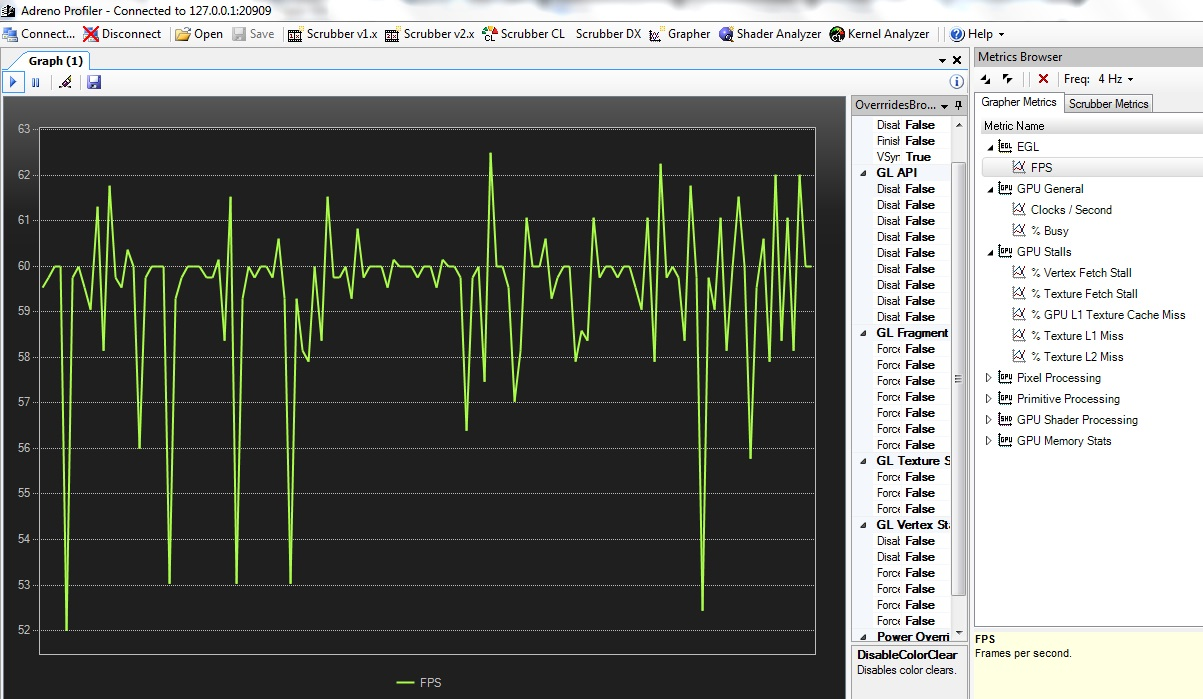
\includegraphics[keepaspectratio=true,scale=0.35]{figuras/graph.jpg}
	\caption{Ferramenta \textit{Adreno Profiler}: quadros por segundo}
	\label{graph}
	\end{figure}


	\item \textbf{2.8.2 \textit{gDEBugger}}
	
	A \textit{gDEBugger} é uma ferramenta de depuração e análise de desempenho (Fig. \ref{gdebugger_fer}), que permite a rastreabilidade das chamadas \textit{OpenGL} de uma aplicação, disponível para \textit{Windows} e \textit{Linux}, com suporte às GPU's da empresa NVIDIA. Ela ajuda a encontrar  \textit{bugs}, melhorar o desempenho e consumo de memória de programas que utilizam a \textit{OpenGL}. 

	Como é mostrado em \cite{gdebugger}, é possível ver quais funções foram chamadas em um determinado quadro, o valor das variáveis da \textit{OpenGL} (como as matrizes de projeção, visualização e modelagem, por exemplo) e também mostrar medições com relação a quadros por segundo, consumo de memória, número de função de chamadas por quadro, entre outros. Além disso, ela (assim como a ferramenta \textit{Adreno Profiler}) também exporta os resultados no formato CSV.  

	\begin{figure}[h]
	\centering
		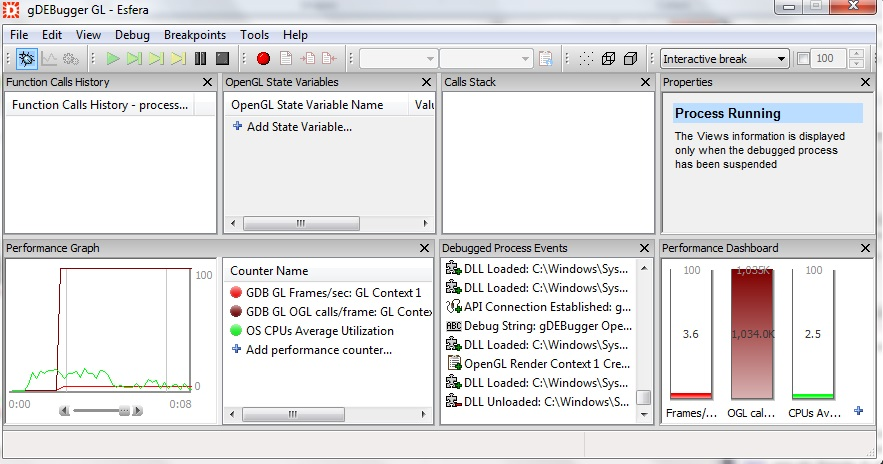
\includegraphics[keepaspectratio=true,scale=0.7]{figuras/gdebugger_fer.jpg}
	\caption{Ferramenta \textit{gDEBugger}: Gráfico de desempenho, histórico de chamadas, valor das variáveis e depuração}
	\label{gdebugger_fer}
	\end{figure}

\end{description} 

\section{Complexidade Algorítmica}

	Complexidade algorítmica é uma medida que compara a eficiência de um determinado algorítmo, analisando o quão custoso ele é,  e foi desenvolvida por Juris Hartmanis e Richard E. Stearns. Segundo  \cite{complexidade}, para não depender do sistema em que está sendo rodado e nem da linguagem de programação, a complexidade algoritmica se baseia em uma função (medida lógica) que expressa uma relação entre a quantidade de dados e de tempo necessário para processá-los.

	 Como o cálculo é relevante somente com relação a grandes quantidades de dados, os termos que não afetam a ordem de magnitude são eliminados e esta aproximação é denominada complexidade assintótica. Assim, a  Eq. 
(\ref{compl1}) poderia ser aproximada pela  Eq. (\ref{compl2})

	\begin{equation}
		y = n^{2} +10 n + 1000
	\label{compl1}
	\end{equation}

	\begin{equation}
		y \approx  n^{2} 
	\label{compl2}
	\end{equation}

	A maioria dos algorítmos possui um parâmetro N (o número de dados a serem processados), que afeta mais significativamente o tempo de execução. De acordo com \cite{complexidade2}, a maioria dos algorítmos se enquadram nos tempos de execução proporcionais aos valores da Tab. (\ref{complexidadeAlgoritmica}) abaixo.

\begin{table}[h]
	\centering	
	\begin{tabular}{cl}
		\toprule
		\textbf{Complexidade} & \textbf{Descrição}  \\
		\midrule
		Constante &  Ocorre quando as instruções do programa \\
		 &  são executadas apenas uma vez.\\
		log N & Ocorre geralmente em programas que resolvem grandes problemas dividindo-os \\
		 &  em partes menores, cortando o seu tamanho por uma constante.  \\
		N & Ocorre quando o programa é linear, ou seja, o \\ 
		 &  processamento é feito para cada elemento de entrada. \\
		$ N log N$ & Ocorre quando o problema é quebrado em partes menores, \\
		 &  sendo resolvidas independentemente, e depois suas soluções são combinadas \\
		$ N^{2}$ & Ocorre quando o algorítmo é quadrático, ou seja, quando \\
		 &  processa todos os pares de itens de dados. \\
		$ N^{3}$ & Ocorre quando o algorítmo é cúbico, ou seja, quando \\
		 &  processa todos as triplas de itens de dados. \\
		$ 2^{N}$ & Ocorre quando o algorítmo segue uma função exponencial, ou seja, \\
		 &  quando o N dobra o tempo de execução vai ao quadrado. \\
	
		\bottomrule
	\end{tabular}
	\caption{ Valores mais comuns de complexidade algorítmica}
	\label{complexidadeAlgoritmica}
\end{table}


\section{Métodos dos Mínimos Quadrados}


	O método dos mínimos quadrados é utilizado para ajustar pontos (x,y) determinados experimentalmente, a uma reta dada por y = a + bx. Faz-se isto, pois muitas vezes estes pontos não são colineares e segundo \cite{minq} é impossível encontrar coeficientes a e b que satisfaçam o sistema. Então, as distâncias destes valores para a reta podem ser consideradas como medidas de erro e os pontos são minimizados pelo mesmo vetor (minimizando a soma dos quadrados destes erros).  Assim, existe um ajuste linear de mínimos quadrados aos dados, e a sua solução é dada pela Eq. (\ref{minquad}).

	\begin{equation}
		v =( M^{T}M)^{-1}M^{T}y
	\label{minquad}
	\end{equation}

	Em que 
	M = $\left[\begin{array}{cc}
               	1 & x1 \\
               	1 & x2  \\
		. & .  \\
               	. & .  \\
		1 & xn
          	         \end{array}\right] \mbox{,} \quad
	v = \left[\begin{array}{c}
               	a \\
               	b  
          	         \end{array}\right] \mbox{e} \quad
	y = \left[\begin{array}{c}
               	y1 \\
               	y2  \\
		.   \\
               	.   \\
		yn
          	         \end{array}\right] $

	Desta forma, é possível determinar os coeficientes a e b e consequentemente, a equação da reta. 
